\documentclass{standalone}
\usepackage{tikz}
\usepackage{ctex,siunitx,fontawesome5}
\setCJKmainfont{Noto Serif CJK SC}
\usepackage{tkz-euclide}
\usepackage{amsmath}
\usetikzlibrary{patterns, calc,3d}
\usetikzlibrary {decorations.pathmorphing,decorations.pathreplacing,decorations.shapes}
\begin{document}
\small
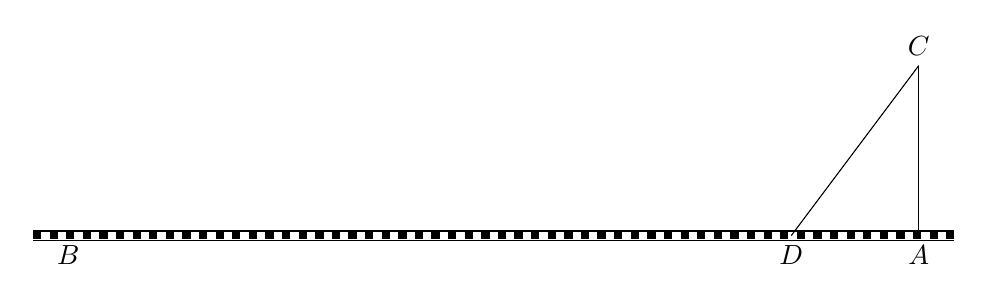
\begin{tikzpicture}[>=latex,scale=0.9]
  \draw[double distance=3pt](-0.5,0)--(12.5,0);
  \draw[line width=2.5pt,dashed](-0.5,0)--(12.5,0);
  \draw(12,0)node[below]{$A$}--(12,2.4)node[above]{$C$};
  \draw(12,2.4)--(10.2,0)node[below]{$D$};
  \node at (0,0)[below]{$B$};
\end{tikzpicture}
\end{document}